\documentclass[UTF8]{ctexart}
\usepackage{graphicx}
\usepackage{float}
\usepackage{subfiles}
\usepackage{pdfpages}
\usepackage[utf8]{inputenc}
\usepackage[english]{babel}
\usepackage{geometry}
\geometry{
	a4paper,
	total={170mm,257mm},
	left=20mm,
	top=20mm
}
\usepackage{listings}

%opening
\title{系统分析与设计方法 \\ 作业 5}
\author{软件42 \\ 欧阳鹏程 \\ 2141601030 \\ 版权声明:Creative Commons BY-NC-ND}

\begin{document}

\maketitle

\begin{enumerate}
	\item 
	系统需求分析与设计:你作为一名软件系统分析员,在某一个高校的学生管理系统中负责系统的分析与设计工作,为了更快地将客户的需求进行建模,你采用了DFD的方法建立了两层数据流模型如下:
	\begin{figure}[H]
		\centering
		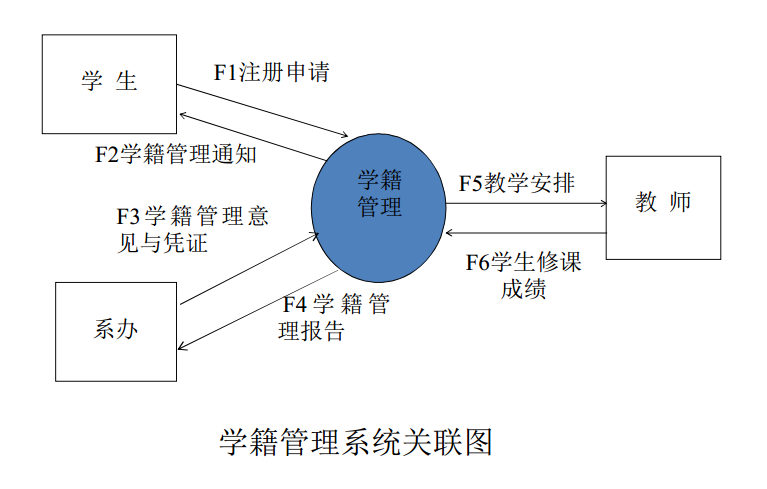
\includegraphics[width=0.7\textwidth]{1}
		\caption{顶层数据流图}
		\label{fig:1}
	\end{figure}
	\begin{figure}[H]
		\centering
		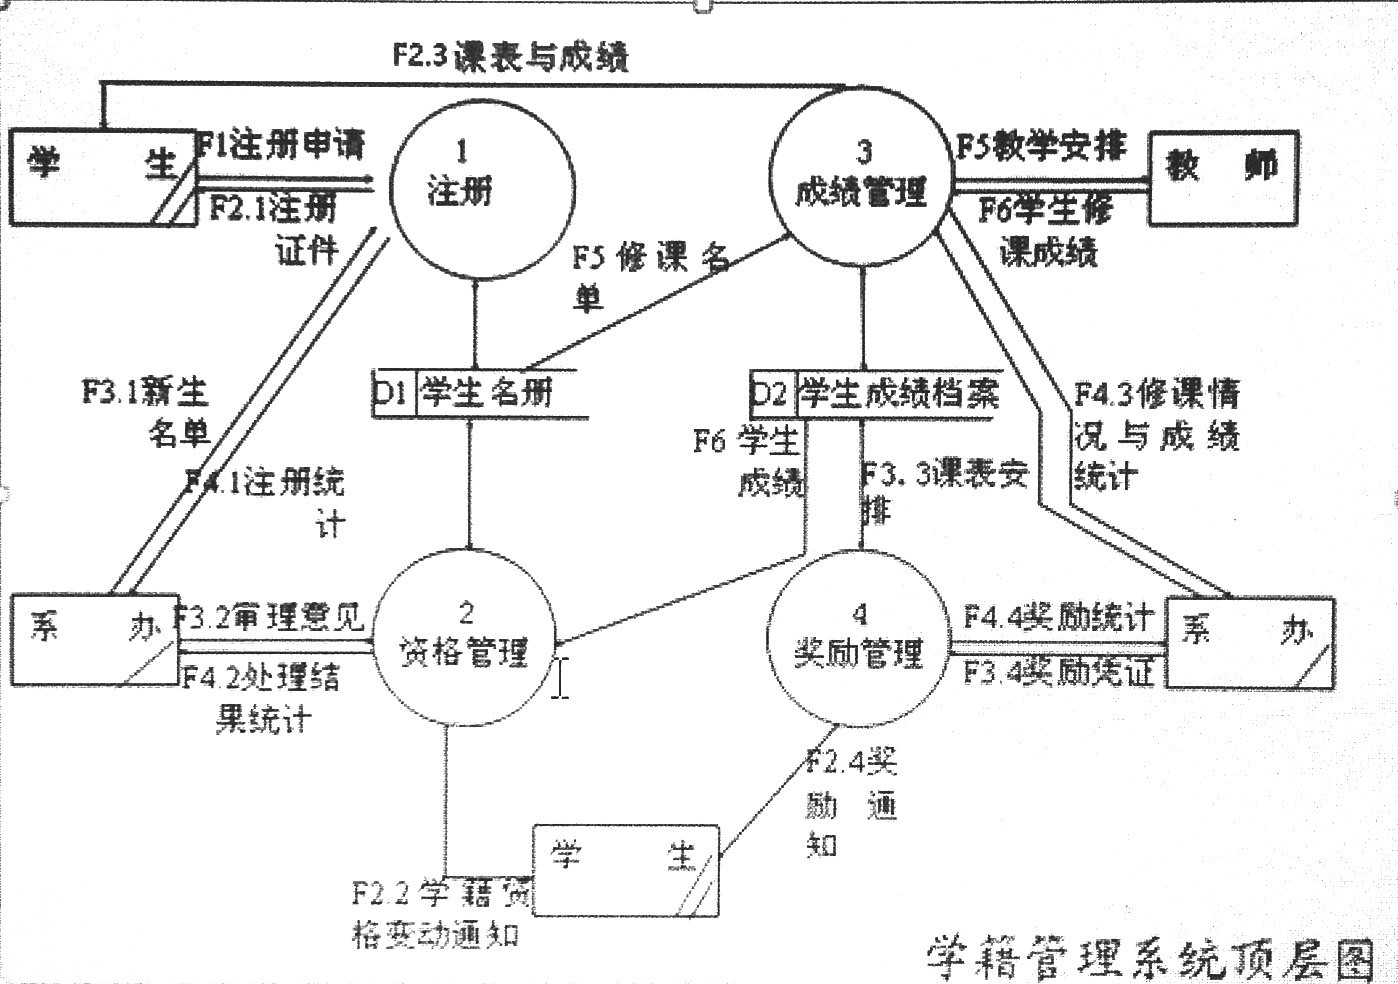
\includegraphics[width=0.7\textwidth]{2}
		\caption{第一层数据流图}
		\label{fig:2}
	\end{figure}
	\begin{itemize}
		\item 问题要求:
		\begin{enumerate}
			\item 但是在与客户经理以及开发人员进行沟通交流时,大家认为这种描述方法已经过时,希望能够采用\textbf{面向对象}的方法来进行业务需求的建模与分析,迫于用户和开发人员的要求,你准备对现有的建模方法进行调整。
			\item 请利用UML的建模方法将该模型转换成等效的功能模型(\textbf{USE CASE图,并简要描述事件流})、动态模型(\textbf{活动图与分析时序图})、以及静态模型(\textbf{分析类图}),\textbf{数据库ER模型},注意说明并解释模型之间存在的关系,且可以根据需要进行扩展,尽量完整和细化。
		\end{enumerate}
	\end{itemize}
	%\subfile{ans.tex}	
\end{enumerate}
\end{document}
